\documentclass[twoside]{book}

% Packages required by doxygen
\usepackage{fixltx2e}
\usepackage{calc}
\usepackage{doxygen}
\usepackage[export]{adjustbox} % also loads graphicx
\usepackage{graphicx}
\usepackage[utf8]{inputenc}
\usepackage{makeidx}
\usepackage{multicol}
\usepackage{multirow}
\PassOptionsToPackage{warn}{textcomp}
\usepackage{textcomp}
\usepackage[nointegrals]{wasysym}
\usepackage[table]{xcolor}

% Font selection
\usepackage[T1]{fontenc}
\usepackage[scaled=.90]{helvet}
\usepackage{courier}
\usepackage{amssymb}
\usepackage{sectsty}
\renewcommand{\familydefault}{\sfdefault}
\allsectionsfont{%
  \fontseries{bc}\selectfont%
  \color{darkgray}%
}
\renewcommand{\DoxyLabelFont}{%
  \fontseries{bc}\selectfont%
  \color{darkgray}%
}
\newcommand{\+}{\discretionary{\mbox{\scriptsize$\hookleftarrow$}}{}{}}

% Page & text layout
\usepackage{geometry}
\geometry{%
  a4paper,%
  top=2.5cm,%
  bottom=2.5cm,%
  left=2.5cm,%
  right=2.5cm%
}
\tolerance=750
\hfuzz=15pt
\hbadness=750
\setlength{\emergencystretch}{15pt}
\setlength{\parindent}{0cm}
\setlength{\parskip}{3ex plus 2ex minus 2ex}
\makeatletter
\renewcommand{\paragraph}{%
  \@startsection{paragraph}{4}{0ex}{-1.0ex}{1.0ex}{%
    \normalfont\normalsize\bfseries\SS@parafont%
  }%
}
\renewcommand{\subparagraph}{%
  \@startsection{subparagraph}{5}{0ex}{-1.0ex}{1.0ex}{%
    \normalfont\normalsize\bfseries\SS@subparafont%
  }%
}
\makeatother

% Headers & footers
\usepackage{fancyhdr}
\pagestyle{fancyplain}
\fancyhead[LE]{\fancyplain{}{\bfseries\thepage}}
\fancyhead[CE]{\fancyplain{}{}}
\fancyhead[RE]{\fancyplain{}{\bfseries\leftmark}}
\fancyhead[LO]{\fancyplain{}{\bfseries\rightmark}}
\fancyhead[CO]{\fancyplain{}{}}
\fancyhead[RO]{\fancyplain{}{\bfseries\thepage}}
\fancyfoot[LE]{\fancyplain{}{}}
\fancyfoot[CE]{\fancyplain{}{}}
\fancyfoot[RE]{\fancyplain{}{\bfseries\scriptsize Generated by Doxygen }}
\fancyfoot[LO]{\fancyplain{}{\bfseries\scriptsize Generated by Doxygen }}
\fancyfoot[CO]{\fancyplain{}{}}
\fancyfoot[RO]{\fancyplain{}{}}
\renewcommand{\footrulewidth}{0.4pt}
\renewcommand{\chaptermark}[1]{%
  \markboth{#1}{}%
}
\renewcommand{\sectionmark}[1]{%
  \markright{\thesection\ #1}%
}

% Indices & bibliography
\usepackage{natbib}
\usepackage[titles]{tocloft}
\setcounter{tocdepth}{3}
\setcounter{secnumdepth}{5}
\makeindex

% Hyperlinks (required, but should be loaded last)
\usepackage{ifpdf}
\ifpdf
  \usepackage[pdftex,pagebackref=true]{hyperref}
\else
  \usepackage[ps2pdf,pagebackref=true]{hyperref}
\fi
\hypersetup{%
  colorlinks=true,%
  linkcolor=blue,%
  citecolor=blue,%
  unicode%
}

% Custom commands
\newcommand{\clearemptydoublepage}{%
  \newpage{\pagestyle{empty}\cleardoublepage}%
}

\usepackage{caption}
\captionsetup{labelsep=space,justification=centering,font={bf},singlelinecheck=off,skip=4pt,position=top}

%===== C O N T E N T S =====

\begin{document}

% Titlepage & ToC
\hypersetup{pageanchor=false,
             bookmarksnumbered=true,
             pdfencoding=unicode
            }
\pagenumbering{alph}
\begin{titlepage}
\vspace*{7cm}
\begin{center}%
{\Large GR S\+DK }\\
\vspace*{1cm}
{\large Generated by Doxygen 1.8.14}\\
\end{center}
\end{titlepage}
\clearemptydoublepage
\pagenumbering{roman}
\tableofcontents
\clearemptydoublepage
\pagenumbering{arabic}
\hypersetup{pageanchor=true}

%--- Begin generated contents ---
\chapter{Hierarchical Index}
\section{Class Hierarchy}
This inheritance list is sorted roughly, but not completely, alphabetically\+:\begin{DoxyCompactList}
\item \contentsline{section}{acc\+\_\+k\+\_\+vars}{\pageref{structacc__k__vars}}{}
\item \contentsline{section}{dbus\+\_\+bluez}{\pageref{structdbus__bluez}}{}
\item \contentsline{section}{dev\+\_\+names}{\pageref{structdev__names}}{}
\item \contentsline{section}{dev\+\_\+socket}{\pageref{structdev__socket}}{}
\item \contentsline{section}{device\+\_\+names}{\pageref{structdevice__names}}{}
\item \contentsline{section}{device\+\_\+t}{\pageref{structdevice__t}}{}
\item \contentsline{section}{device\+\_\+uuids}{\pageref{structdevice__uuids}}{}
\item \contentsline{section}{finger}{\pageref{structfinger}}{}
\item \contentsline{section}{Gestus\+Connection}{\pageref{classGestusConnection}}{}
\item \contentsline{section}{G\+N\+U\+Plot}{\pageref{classGNUPlot}}{}
\item \contentsline{section}{gr\+\_\+alg\+\_\+message}{\pageref{structgr__alg__message}}{}
\item \contentsline{section}{gr\+\_\+message}{\pageref{structgr__message}}{}
\item \contentsline{section}{G\+R\+Connection}{\pageref{classGRConnection}}{}
\item \contentsline{section}{G\+R\+Grt}{\pageref{classGRGrt}}{}
\begin{DoxyCompactList}
\item \contentsline{section}{G\+R\+Algorithm}{\pageref{classGRAlgorithm}}{}
\item \contentsline{section}{G\+R\+Utilities}{\pageref{classGRUtilities}}{}
\end{DoxyCompactList}
\item \contentsline{section}{G\+R\+Madgwick}{\pageref{classGRMadgwick}}{}
\item \contentsline{section}{G\+R\+Trajectory}{\pageref{classGRTrajectory}}{}
\item \contentsline{section}{imu}{\pageref{structimu}}{}
\item \contentsline{section}{k\+\_\+filter\+\_\+vars}{\pageref{structk__filter__vars}}{}
\item \contentsline{section}{runge\+\_\+vars}{\pageref{structrunge__vars}}{}
\end{DoxyCompactList}

\chapter{Class Index}
\section{Class List}
Here are the classes, structs, unions and interfaces with brief descriptions\+:\begin{DoxyCompactList}
\item\contentsline{section}{\mbox{\hyperlink{structacc__k__vars}{acc\+\_\+k\+\_\+vars}} }{\pageref{structacc__k__vars}}{}
\item\contentsline{section}{\mbox{\hyperlink{structdbus__bluez}{dbus\+\_\+bluez}} }{\pageref{structdbus__bluez}}{}
\item\contentsline{section}{\mbox{\hyperlink{structdev__names}{dev\+\_\+names}} }{\pageref{structdev__names}}{}
\item\contentsline{section}{\mbox{\hyperlink{structdev__socket}{dev\+\_\+socket}} }{\pageref{structdev__socket}}{}
\item\contentsline{section}{\mbox{\hyperlink{structdevice__names}{device\+\_\+names}} }{\pageref{structdevice__names}}{}
\item\contentsline{section}{\mbox{\hyperlink{structdevice__t}{device\+\_\+t}} }{\pageref{structdevice__t}}{}
\item\contentsline{section}{\mbox{\hyperlink{structdevice__uuids}{device\+\_\+uuids}} }{\pageref{structdevice__uuids}}{}
\item\contentsline{section}{\mbox{\hyperlink{structfinger}{finger}} }{\pageref{structfinger}}{}
\item\contentsline{section}{\mbox{\hyperlink{classGestusConnection}{Gestus\+Connection}} }{\pageref{classGestusConnection}}{}
\item\contentsline{section}{\mbox{\hyperlink{classGNUPlot}{G\+N\+U\+Plot}} }{\pageref{classGNUPlot}}{}
\item\contentsline{section}{\mbox{\hyperlink{structgr__alg__message}{gr\+\_\+alg\+\_\+message}} }{\pageref{structgr__alg__message}}{}
\item\contentsline{section}{\mbox{\hyperlink{structgr__message}{gr\+\_\+message}} }{\pageref{structgr__message}}{}
\item\contentsline{section}{\mbox{\hyperlink{classGRAlgorithm}{G\+R\+Algorithm}} }{\pageref{classGRAlgorithm}}{}
\item\contentsline{section}{\mbox{\hyperlink{classGRConnection}{G\+R\+Connection}} }{\pageref{classGRConnection}}{}
\item\contentsline{section}{\mbox{\hyperlink{classGRGrt}{G\+R\+Grt}} }{\pageref{classGRGrt}}{}
\item\contentsline{section}{\mbox{\hyperlink{classGRMadgwick}{G\+R\+Madgwick}} }{\pageref{classGRMadgwick}}{}
\item\contentsline{section}{\mbox{\hyperlink{classGRTrajectory}{G\+R\+Trajectory}} }{\pageref{classGRTrajectory}}{}
\item\contentsline{section}{\mbox{\hyperlink{classGRUtilities}{G\+R\+Utilities}} }{\pageref{classGRUtilities}}{}
\item\contentsline{section}{\mbox{\hyperlink{structimu}{imu}} }{\pageref{structimu}}{}
\item\contentsline{section}{\mbox{\hyperlink{structk__filter__vars}{k\+\_\+filter\+\_\+vars}} }{\pageref{structk__filter__vars}}{}
\item\contentsline{section}{\mbox{\hyperlink{structrunge__vars}{runge\+\_\+vars}} }{\pageref{structrunge__vars}}{}
\end{DoxyCompactList}

\chapter{Class Documentation}
\hypertarget{structacc__k__vars}{}\section{acc\+\_\+k\+\_\+vars Struct Reference}
\label{structacc__k__vars}\index{acc\+\_\+k\+\_\+vars@{acc\+\_\+k\+\_\+vars}}
\subsection*{Public Attributes}
\begin{DoxyCompactItemize}
\item 
\mbox{\Hypertarget{structacc__k__vars_a8520459b0302db23887ae66a172d803e}\label{structacc__k__vars_a8520459b0302db23887ae66a172d803e}} 
\mbox{\hyperlink{structk__filter__vars}{k\+\_\+filter\+\_\+vars}} {\bfseries acc\+\_\+k\+\_\+x}
\item 
\mbox{\Hypertarget{structacc__k__vars_a2e819b3166338fe86a3ef7c3ab7f0636}\label{structacc__k__vars_a2e819b3166338fe86a3ef7c3ab7f0636}} 
\mbox{\hyperlink{structk__filter__vars}{k\+\_\+filter\+\_\+vars}} {\bfseries acc\+\_\+k\+\_\+y}
\item 
\mbox{\Hypertarget{structacc__k__vars_aa10974f1bd2776c2ffc0a577e88e213f}\label{structacc__k__vars_aa10974f1bd2776c2ffc0a577e88e213f}} 
\mbox{\hyperlink{structk__filter__vars}{k\+\_\+filter\+\_\+vars}} {\bfseries acc\+\_\+k\+\_\+z}
\end{DoxyCompactItemize}


The documentation for this struct was generated from the following file\+:\begin{DoxyCompactItemize}
\item 
/home/vlad/projects/brainhub/gestus\+S\+D\+K/inc/gr\+Algorithm.\+h\end{DoxyCompactItemize}

\hypertarget{structdbus__bluez}{}\section{dbus\+\_\+bluez Struct Reference}
\label{structdbus__bluez}\index{dbus\+\_\+bluez@{dbus\+\_\+bluez}}
\subsection*{Public Attributes}
\begin{DoxyCompactItemize}
\item 
\mbox{\Hypertarget{structdbus__bluez_a53fba2b3c8bbc075353364ad983decb7}\label{structdbus__bluez_a53fba2b3c8bbc075353364ad983decb7}} 
std\+::string {\bfseries name}
\item 
\mbox{\Hypertarget{structdbus__bluez_a06562a13c9877c5bfcb4aa3796f8afdd}\label{structdbus__bluez_a06562a13c9877c5bfcb4aa3796f8afdd}} 
std\+::string {\bfseries path}
\item 
\mbox{\Hypertarget{structdbus__bluez_ac2590c9e985831da2d117cafeb51fa9e}\label{structdbus__bluez_ac2590c9e985831da2d117cafeb51fa9e}} 
std\+::string {\bfseries properties}
\item 
\mbox{\Hypertarget{structdbus__bluez_a739d986ed0b243fb486bb78ce1a201fb}\label{structdbus__bluez_a739d986ed0b243fb486bb78ce1a201fb}} 
std\+::string {\bfseries introspectable}
\end{DoxyCompactItemize}


The documentation for this struct was generated from the following file\+:\begin{DoxyCompactItemize}
\item 
/home/vlad/projects/brainhub/gestus\+S\+D\+K/experimental/gr\+L\+E\+Bluez\+Attributes.\+h\end{DoxyCompactItemize}

\hypertarget{structdev__names}{}\section{dev\+\_\+names Struct Reference}
\label{structdev__names}\index{dev\+\_\+names@{dev\+\_\+names}}
\subsection*{Public Attributes}
\begin{DoxyCompactItemize}
\item 
\mbox{\Hypertarget{structdev__names_a7030548518cf451ccb9dc115e944101c}\label{structdev__names_a7030548518cf451ccb9dc115e944101c}} 
std\+::string {\bfseries left}
\item 
\mbox{\Hypertarget{structdev__names_a9ae36fcd43bf07d10041b6d4d1c874b7}\label{structdev__names_a9ae36fcd43bf07d10041b6d4d1c874b7}} 
std\+::string {\bfseries right}
\item 
\mbox{\Hypertarget{structdev__names_ad0c0d1c45c95408489fa9981b77191ea}\label{structdev__names_ad0c0d1c45c95408489fa9981b77191ea}} 
std\+::string {\bfseries test}
\end{DoxyCompactItemize}


The documentation for this struct was generated from the following file\+:\begin{DoxyCompactItemize}
\item 
/home/vlad/projects/brainhub/gestus\+S\+D\+K/inc/gr\+Device.\+h\end{DoxyCompactItemize}

\hypertarget{structdev__socket}{}\section{dev\+\_\+socket Struct Reference}
\label{structdev__socket}\index{dev\+\_\+socket@{dev\+\_\+socket}}
\subsection*{Public Member Functions}
\begin{DoxyCompactItemize}
\item 
\mbox{\Hypertarget{structdev__socket_ad1876873738658ed76347fde5f70c1eb}\label{structdev__socket_ad1876873738658ed76347fde5f70c1eb}} 
sockaddr\+\_\+rc $\ast$ {\bfseries get\+Addr\+Ref} ()
\end{DoxyCompactItemize}
\subsection*{Public Attributes}
\begin{DoxyCompactItemize}
\item 
\mbox{\Hypertarget{structdev__socket_a8bc6d848be0a9f4ec7d7639ac66eb932}\label{structdev__socket_a8bc6d848be0a9f4ec7d7639ac66eb932}} 
int {\bfseries sock}
\item 
\mbox{\Hypertarget{structdev__socket_aa49a0dec9aebbdff2482f5bfb81b2b52}\label{structdev__socket_aa49a0dec9aebbdff2482f5bfb81b2b52}} 
struct sockaddr\+\_\+rc {\bfseries addr} = \{ 0 \}
\end{DoxyCompactItemize}


The documentation for this struct was generated from the following file\+:\begin{DoxyCompactItemize}
\item 
/home/vlad/projects/brainhub/gestus\+S\+D\+K/inc/gr\+Connection.\+h\end{DoxyCompactItemize}

\hypertarget{structdevice__names}{}\section{device\+\_\+names Struct Reference}
\label{structdevice__names}\index{device\+\_\+names@{device\+\_\+names}}
\subsection*{Public Attributes}
\begin{DoxyCompactItemize}
\item 
\mbox{\Hypertarget{structdevice__names_a2bb27860a20d44acaa75c72aa24081e0}\label{structdevice__names_a2bb27860a20d44acaa75c72aa24081e0}} 
std\+::string {\bfseries left}
\item 
\mbox{\Hypertarget{structdevice__names_a54a02fec078cf2f0b4456c0febaf0694}\label{structdevice__names_a54a02fec078cf2f0b4456c0febaf0694}} 
std\+::string {\bfseries right}
\end{DoxyCompactItemize}


The documentation for this struct was generated from the following file\+:\begin{DoxyCompactItemize}
\item 
/home/vlad/projects/brainhub/gestus\+S\+D\+K/experimental/gr\+L\+E\+Bluez\+Attributes.\+h\end{DoxyCompactItemize}

\hypertarget{structdevice__t}{}\section{device\+\_\+t Struct Reference}
\label{structdevice__t}\index{device\+\_\+t@{device\+\_\+t}}
\subsection*{Public Member Functions}
\begin{DoxyCompactItemize}
\item 
\mbox{\Hypertarget{structdevice__t_ac77b0b37f8860be8c8ea2fc236e831c2}\label{structdevice__t_ac77b0b37f8860be8c8ea2fc236e831c2}} 
void {\bfseries clear\+\_\+attributes} ()
\end{DoxyCompactItemize}
\subsection*{Public Attributes}
\begin{DoxyCompactItemize}
\item 
\mbox{\Hypertarget{structdevice__t_ab6fb06faaf77e3218eba621ce4b9e156}\label{structdevice__t_ab6fb06faaf77e3218eba621ce4b9e156}} 
int {\bfseries id}
\item 
\mbox{\Hypertarget{structdevice__t_adb384c5c8cb489d608dcb7b80a40b52c}\label{structdevice__t_adb384c5c8cb489d608dcb7b80a40b52c}} 
std\+::string {\bfseries name}
\item 
\mbox{\Hypertarget{structdevice__t_a3ebddb374c44b31ada528da828e0bcdf}\label{structdevice__t_a3ebddb374c44b31ada528da828e0bcdf}} 
std\+::string {\bfseries address}
\end{DoxyCompactItemize}


The documentation for this struct was generated from the following file\+:\begin{DoxyCompactItemize}
\item 
/home/vlad/projects/brainhub/gestus\+S\+D\+K/inc/gr\+Device.\+h\end{DoxyCompactItemize}

\hypertarget{structdevice__uuids}{}\section{device\+\_\+uuids Struct Reference}
\label{structdevice__uuids}\index{device\+\_\+uuids@{device\+\_\+uuids}}
\subsection*{Public Attributes}
\begin{DoxyCompactItemize}
\item 
\mbox{\Hypertarget{structdevice__uuids_a97d5ed5abadd8a616af4ff63ca04abb7}\label{structdevice__uuids_a97d5ed5abadd8a616af4ff63ca04abb7}} 
\mbox{\hyperlink{structfinger}{finger}} {\bfseries fingers} \mbox{[}5\mbox{]}
\item 
\mbox{\Hypertarget{structdevice__uuids_ac693aab2b40e74989e0263611d3aeaa6}\label{structdevice__uuids_ac693aab2b40e74989e0263611d3aeaa6}} 
std\+::string {\bfseries gyro}
\item 
\mbox{\Hypertarget{structdevice__uuids_a64e32986e00d0e2e17b0a7c483fd4ab4}\label{structdevice__uuids_a64e32986e00d0e2e17b0a7c483fd4ab4}} 
std\+::string {\bfseries accelerometer}
\item 
\mbox{\Hypertarget{structdevice__uuids_aa7c316bf72656b77ce08940bd163d863}\label{structdevice__uuids_aa7c316bf72656b77ce08940bd163d863}} 
std\+::string {\bfseries magnet}
\item 
\mbox{\Hypertarget{structdevice__uuids_ac2dad171c756ef00fbda3bb436046395}\label{structdevice__uuids_ac2dad171c756ef00fbda3bb436046395}} 
std\+::string {\bfseries rx}
\item 
\mbox{\Hypertarget{structdevice__uuids_a35e3ec1e919eee33abe7871287830637}\label{structdevice__uuids_a35e3ec1e919eee33abe7871287830637}} 
std\+::string {\bfseries tx}
\item 
\mbox{\Hypertarget{structdevice__uuids_ab93540c7489b327f629a83b623b24988}\label{structdevice__uuids_ab93540c7489b327f629a83b623b24988}} 
std\+::string {\bfseries tmp\+\_\+uuid}
\end{DoxyCompactItemize}


The documentation for this struct was generated from the following file\+:\begin{DoxyCompactItemize}
\item 
/home/vlad/projects/brainhub/gestus\+S\+D\+K/experimental/gr\+L\+E\+Bluez\+Attributes.\+h\end{DoxyCompactItemize}

\hypertarget{structfinger}{}\section{finger Struct Reference}
\label{structfinger}\index{finger@{finger}}
\subsection*{Public Attributes}
\begin{DoxyCompactItemize}
\item 
\mbox{\Hypertarget{structfinger_ae76d8541ff4d95b40806d4e12ae1e25d}\label{structfinger_ae76d8541ff4d95b40806d4e12ae1e25d}} 
std\+::string {\bfseries gyro}
\item 
\mbox{\Hypertarget{structfinger_a35e626569c38aeb7b37fae94cf4c210a}\label{structfinger_a35e626569c38aeb7b37fae94cf4c210a}} 
std\+::string {\bfseries accelerometer}
\item 
\mbox{\Hypertarget{structfinger_a65194f954de07e809a5048c7d2412fd7}\label{structfinger_a65194f954de07e809a5048c7d2412fd7}} 
std\+::string {\bfseries mag}
\end{DoxyCompactItemize}


The documentation for this struct was generated from the following file\+:\begin{DoxyCompactItemize}
\item 
/home/vlad/projects/brainhub/gestus\+S\+D\+K/experimental/gr\+L\+E\+Bluez\+Attributes.\+h\end{DoxyCompactItemize}

\hypertarget{classGestusConnection}{}\section{Gestus\+Connection Class Reference}
\label{classGestusConnection}\index{Gestus\+Connection@{Gestus\+Connection}}
\subsection*{Public Member Functions}
\begin{DoxyCompactItemize}
\item 
\mbox{\Hypertarget{classGestusConnection_a1dd64b164bff6ee4d8a49406bc9582b5}\label{classGestusConnection_a1dd64b164bff6ee4d8a49406bc9582b5}} 
{\bfseries Gestus\+Connection} (const \mbox{\hyperlink{classGestusConnection}{Gestus\+Connection}} \&)
\item 
\mbox{\Hypertarget{classGestusConnection_a6a83fb5fa1ca84e37206c223fe382925}\label{classGestusConnection_a6a83fb5fa1ca84e37206c223fe382925}} 
\mbox{\hyperlink{classGestusConnection}{Gestus\+Connection}} \& {\bfseries operator=} (const \mbox{\hyperlink{classGestusConnection}{Gestus\+Connection}} \&)
\item 
\mbox{\Hypertarget{classGestusConnection_acc086565d3a371b5b3aa1536df336606}\label{classGestusConnection_acc086565d3a371b5b3aa1536df336606}} 
bool {\bfseries set\+Adapter\+Name} ()
\item 
\mbox{\Hypertarget{classGestusConnection_a62623bbcaed138c5c26d9f2509a02dbe}\label{classGestusConnection_a62623bbcaed138c5c26d9f2509a02dbe}} 
std\+::string {\bfseries get\+Adapter\+Name} ()
\item 
\mbox{\Hypertarget{classGestusConnection_a2d94def208a11c30ecdd8cd5464730d6}\label{classGestusConnection_a2d94def208a11c30ecdd8cd5464730d6}} 
\mbox{\hyperlink{structdevice__t}{device\+\_\+t}} {\bfseries get\+Adapter} ()
\item 
\mbox{\Hypertarget{classGestusConnection_a22050dece0a420bdacb4c7d59c87954d}\label{classGestusConnection_a22050dece0a420bdacb4c7d59c87954d}} 
int {\bfseries get\+Device\+Id} (\mbox{\hyperlink{structdevice__t}{device\+\_\+t}})
\item 
\mbox{\Hypertarget{classGestusConnection_aafaade299ab1579a328270adf9f395e7}\label{classGestusConnection_aafaade299ab1579a328270adf9f395e7}} 
std\+::string {\bfseries get\+Device\+Name} (\mbox{\hyperlink{structdevice__t}{device\+\_\+t}})
\item 
\mbox{\Hypertarget{classGestusConnection_ad453799d5224e34f41859b7d6265d9ef}\label{classGestusConnection_ad453799d5224e34f41859b7d6265d9ef}} 
std\+::vector$<$ \mbox{\hyperlink{structdevice__t}{device\+\_\+t}} $>$ {\bfseries get\+Connected\+Devices} ()
\item 
\mbox{\Hypertarget{classGestusConnection_a8aa58479a29e3b3a016abb6e61117c67}\label{classGestusConnection_a8aa58479a29e3b3a016abb6e61117c67}} 
bool {\bfseries get\+Data} (int, std\+::string, std\+::deque$<$ std\+::string $>$ $\ast$)
\item 
\mbox{\Hypertarget{classGestusConnection_acf7376b8f748afb08905b4dcf3a92504}\label{classGestusConnection_acf7376b8f748afb08905b4dcf3a92504}} 
bool {\bfseries connect\+And\+Read} (\mbox{\hyperlink{structdevice__t}{device\+\_\+t}}, std\+::string, std\+::deque$<$ std\+::string $>$ $\ast$)
\item 
\mbox{\Hypertarget{classGestusConnection_a33c945ff8132d2f273bef9c5d5e92626}\label{classGestusConnection_a33c945ff8132d2f273bef9c5d5e92626}} 
bool {\bfseries set\+Avalible\+Devices} ()
\end{DoxyCompactItemize}


The documentation for this class was generated from the following file\+:\begin{DoxyCompactItemize}
\item 
/home/vlad/projects/brainhub/gestus\+S\+D\+K/experimental/gestus\+L\+E\+Connection.\+h\end{DoxyCompactItemize}

\hypertarget{classGNUPlot}{}\section{G\+N\+U\+Plot Class Reference}
\label{classGNUPlot}\index{G\+N\+U\+Plot@{G\+N\+U\+Plot}}
\subsection*{Public Member Functions}
\begin{DoxyCompactItemize}
\item 
\mbox{\Hypertarget{classGNUPlot_a0564d60ca411f0d7fe794e34dcd68ecf}\label{classGNUPlot_a0564d60ca411f0d7fe794e34dcd68ecf}} 
bool {\bfseries is\+Opened} () const
\item 
\mbox{\Hypertarget{classGNUPlot_a186ea2fed8f547252fd5db8e38660f1a}\label{classGNUPlot_a186ea2fed8f547252fd5db8e38660f1a}} 
void {\bfseries open} ()
\item 
\mbox{\Hypertarget{classGNUPlot_ad6185af970ebace0913d8331c56eaebd}\label{classGNUPlot_ad6185af970ebace0913d8331c56eaebd}} 
void {\bfseries flush} ()
\item 
\mbox{\Hypertarget{classGNUPlot_ab27c2ecae2068830d0e8c971d44bd676}\label{classGNUPlot_ab27c2ecae2068830d0e8c971d44bd676}} 
void {\bfseries close} ()
\item 
\mbox{\Hypertarget{classGNUPlot_a2a229273dcf77c882931c8bd508cc909}\label{classGNUPlot_a2a229273dcf77c882931c8bd508cc909}} 
void {\bfseries write} (const char $\ast$line)
\item 
\mbox{\Hypertarget{classGNUPlot_a42f713638f21a023e3dcebe013f431b4}\label{classGNUPlot_a42f713638f21a023e3dcebe013f431b4}} 
void {\bfseries write} (const std\+::string \&line)
\item 
\mbox{\Hypertarget{classGNUPlot_a2774d4b9d63931b48aee47a1dbe55c96}\label{classGNUPlot_a2774d4b9d63931b48aee47a1dbe55c96}} 
void {\bfseries execute} (const std\+::vector$<$ std\+::string $>$ \&script)
\end{DoxyCompactItemize}


The documentation for this class was generated from the following files\+:\begin{DoxyCompactItemize}
\item 
/home/vlad/projects/brainhub/gestus\+S\+D\+K/inc/G\+N\+U\+Plot.\+h\item 
/home/vlad/projects/brainhub/gestus\+S\+D\+K/src/G\+N\+U\+Plot.\+cpp\end{DoxyCompactItemize}

\hypertarget{structgr__alg__message}{}\section{gr\+\_\+alg\+\_\+message Struct Reference}
\label{structgr__alg__message}\index{gr\+\_\+alg\+\_\+message@{gr\+\_\+alg\+\_\+message}}
\subsection*{Public Member Functions}
\begin{DoxyCompactItemize}
\item 
\mbox{\Hypertarget{structgr__alg__message_a2eca0bdd161d85e3915019782ab3c7d0}\label{structgr__alg__message_a2eca0bdd161d85e3915019782ab3c7d0}} 
bool {\bfseries clear} ()
\end{DoxyCompactItemize}
\subsection*{Public Attributes}
\begin{DoxyCompactItemize}
\item 
\mbox{\Hypertarget{structgr__alg__message_affba38c037a598035da63f74b679ba7d}\label{structgr__alg__message_affba38c037a598035da63f74b679ba7d}} 
std\+::vector$<$ double $>$ {\bfseries pinky}
\item 
\mbox{\Hypertarget{structgr__alg__message_a41f038022b78c8177a0973ee0d904311}\label{structgr__alg__message_a41f038022b78c8177a0973ee0d904311}} 
std\+::vector$<$ double $>$ {\bfseries ring}
\item 
\mbox{\Hypertarget{structgr__alg__message_ab8bf9a84283523061d9b7c81ad6275a9}\label{structgr__alg__message_ab8bf9a84283523061d9b7c81ad6275a9}} 
std\+::vector$<$ double $>$ {\bfseries middle}
\item 
\mbox{\Hypertarget{structgr__alg__message_a386ca5c0b3cbb207e8d448b38c52a88b}\label{structgr__alg__message_a386ca5c0b3cbb207e8d448b38c52a88b}} 
std\+::vector$<$ double $>$ {\bfseries index}
\item 
\mbox{\Hypertarget{structgr__alg__message_a8273f9f907dbbd1807853632eec80920}\label{structgr__alg__message_a8273f9f907dbbd1807853632eec80920}} 
std\+::vector$<$ double $>$ {\bfseries thumb}
\item 
\mbox{\Hypertarget{structgr__alg__message_aab7d06cfa17d559516adf6afd2bc7829}\label{structgr__alg__message_aab7d06cfa17d559516adf6afd2bc7829}} 
std\+::vector$<$ double $>$ {\bfseries palm}
\item 
\mbox{\Hypertarget{structgr__alg__message_ad3c2b4fc2608141605baa03b5c0e6f9a}\label{structgr__alg__message_ad3c2b4fc2608141605baa03b5c0e6f9a}} 
std\+::unordered\+\_\+map$<$ std\+::string, std\+::vector$<$ double $>$ $\ast$ $>$ {\bfseries nodes}
\end{DoxyCompactItemize}


The documentation for this struct was generated from the following file\+:\begin{DoxyCompactItemize}
\item 
/home/vlad/projects/brainhub/gestus\+S\+D\+K/inc/gr\+Device.\+h\end{DoxyCompactItemize}

\hypertarget{structgr__message}{}\section{gr\+\_\+message Struct Reference}
\label{structgr__message}\index{gr\+\_\+message@{gr\+\_\+message}}
\subsection*{Public Member Functions}
\begin{DoxyCompactItemize}
\item 
\mbox{\Hypertarget{structgr__message_ab1df69a5188f8c594e5c3116bc1e2f2a}\label{structgr__message_ab1df69a5188f8c594e5c3116bc1e2f2a}} 
bool {\bfseries clear} ()
\end{DoxyCompactItemize}
\subsection*{Public Attributes}
\begin{DoxyCompactItemize}
\item 
\mbox{\Hypertarget{structgr__message_a3725100d9e5d207cceecc5f5308d78a0}\label{structgr__message_a3725100d9e5d207cceecc5f5308d78a0}} 
int {\bfseries id}
\item 
\mbox{\Hypertarget{structgr__message_a89059be54c454b6e595ec1edc2221e09}\label{structgr__message_a89059be54c454b6e595ec1edc2221e09}} 
\mbox{\hyperlink{structimu}{imu}} {\bfseries pinky}
\item 
\mbox{\Hypertarget{structgr__message_a46cf80604fac242307667a5b84191d8c}\label{structgr__message_a46cf80604fac242307667a5b84191d8c}} 
\mbox{\hyperlink{structimu}{imu}} {\bfseries ring}
\item 
\mbox{\Hypertarget{structgr__message_ad064db84aad78718a0fa49b269a7cff6}\label{structgr__message_ad064db84aad78718a0fa49b269a7cff6}} 
\mbox{\hyperlink{structimu}{imu}} {\bfseries middle}
\item 
\mbox{\Hypertarget{structgr__message_a7a1bf7b6f5ef36909d9367419a3aaece}\label{structgr__message_a7a1bf7b6f5ef36909d9367419a3aaece}} 
\mbox{\hyperlink{structimu}{imu}} {\bfseries index}
\item 
\mbox{\Hypertarget{structgr__message_ae414ed9059d5def115c26a370d92fc6e}\label{structgr__message_ae414ed9059d5def115c26a370d92fc6e}} 
\mbox{\hyperlink{structimu}{imu}} {\bfseries thumb}
\item 
\mbox{\Hypertarget{structgr__message_a2cba19162c0f25b6191827ea20c55d29}\label{structgr__message_a2cba19162c0f25b6191827ea20c55d29}} 
\mbox{\hyperlink{structimu}{imu}} {\bfseries palm}
\item 
\mbox{\Hypertarget{structgr__message_a6d67d3ee727d1ed7bd28cd765ed9cb72}\label{structgr__message_a6d67d3ee727d1ed7bd28cd765ed9cb72}} 
std\+::unordered\+\_\+map$<$ std\+::string, \mbox{\hyperlink{structimu}{imu}} $\ast$ $>$ {\bfseries imus}
\end{DoxyCompactItemize}


The documentation for this struct was generated from the following file\+:\begin{DoxyCompactItemize}
\item 
/home/vlad/projects/brainhub/gestus\+S\+D\+K/inc/gr\+Device.\+h\end{DoxyCompactItemize}

\hypertarget{classGRAlgorithm}{}\section{G\+R\+Algorithm Class Reference}
\label{classGRAlgorithm}\index{G\+R\+Algorithm@{G\+R\+Algorithm}}
Inheritance diagram for G\+R\+Algorithm\+:\begin{figure}[H]
\begin{center}
\leavevmode
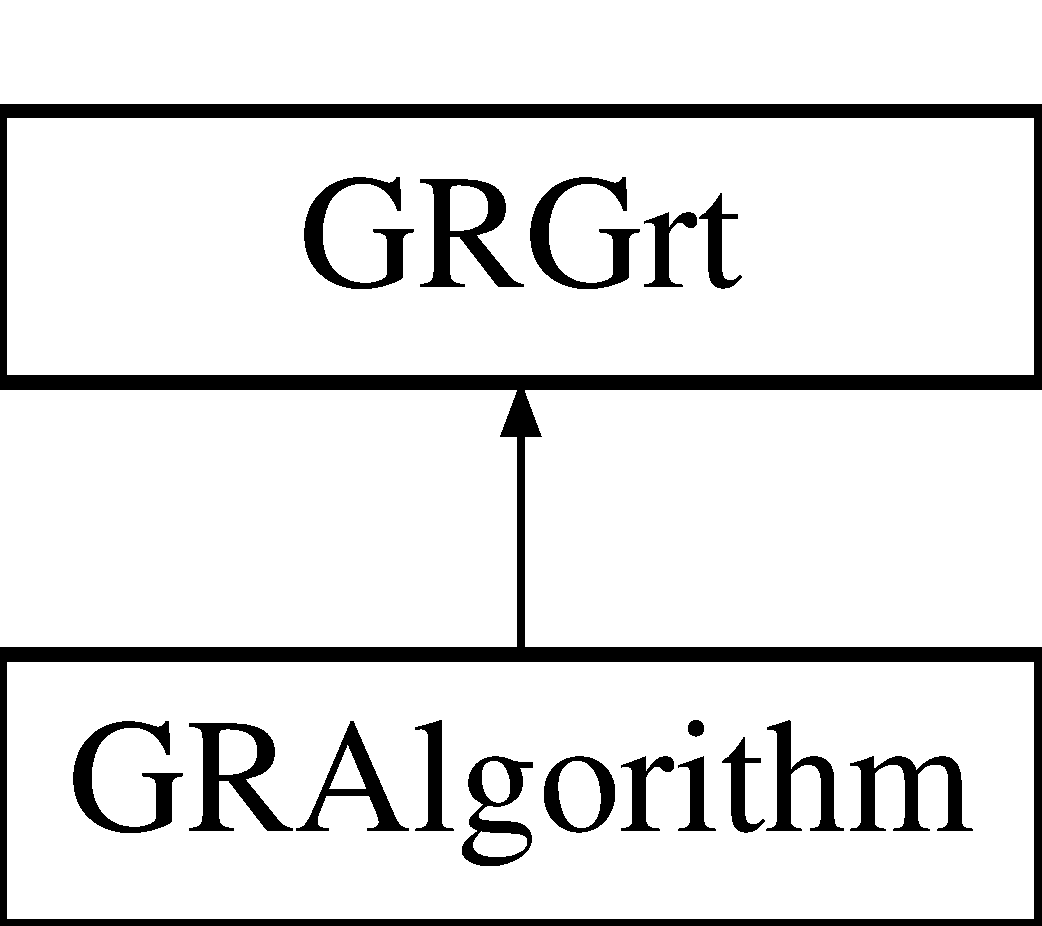
\includegraphics[height=2.000000cm]{classGRAlgorithm}
\end{center}
\end{figure}
\subsection*{Public Member Functions}
\begin{DoxyCompactItemize}
\item 
\mbox{\Hypertarget{classGRAlgorithm_ad507e4837f87aa62d71dcecdca81529e}\label{classGRAlgorithm_ad507e4837f87aa62d71dcecdca81529e}} 
{\bfseries G\+R\+Algorithm} (const \mbox{\hyperlink{classGRAlgorithm}{G\+R\+Algorithm}} \&)
\item 
\mbox{\Hypertarget{classGRAlgorithm_a4ac1b56a7745066e5b046199747ba9ce}\label{classGRAlgorithm_a4ac1b56a7745066e5b046199747ba9ce}} 
\mbox{\hyperlink{classGRAlgorithm}{G\+R\+Algorithm}} \& {\bfseries operator=} (const \mbox{\hyperlink{classGRAlgorithm}{G\+R\+Algorithm}} \&)
\item 
\mbox{\Hypertarget{classGRAlgorithm_aa088e3919a405f830dce381f7b264606}\label{classGRAlgorithm_aa088e3919a405f830dce381f7b264606}} 
void {\bfseries gr\+Init\+Algorithms} ()
\item 
\mbox{\Hypertarget{classGRAlgorithm_a99d42de12749f53522f0bb3b470b876c}\label{classGRAlgorithm_a99d42de12749f53522f0bb3b470b876c}} 
bool {\bfseries madgwick\+Update} (\mbox{\hyperlink{structgr__message}{gr\+\_\+message}} $\ast$, \mbox{\hyperlink{structgr__alg__message}{gr\+\_\+alg\+\_\+message}} $\ast$, int, std\+::string flag)
\item 
\mbox{\Hypertarget{classGRAlgorithm_a4dcbcdb9e123d4b406a44cbc0f7967c1}\label{classGRAlgorithm_a4dcbcdb9e123d4b406a44cbc0f7967c1}} 
bool {\bfseries setup\+Madgwick} (int, int, int, int, int, int)
\item 
\mbox{\Hypertarget{classGRAlgorithm_af66f5bd468eef3647bd8df8942df2470}\label{classGRAlgorithm_af66f5bd468eef3647bd8df8942df2470}} 
bool {\bfseries set\+Up\+Kfilter} (std\+::vector$<$ Eigen\+::\+Vector3d $>$, \mbox{\hyperlink{structacc__k__vars}{acc\+\_\+k\+\_\+vars}} $\ast$)
\item 
\mbox{\Hypertarget{classGRAlgorithm_a23e089dbd28adfe3e36dba5ecd02dd0a}\label{classGRAlgorithm_a23e089dbd28adfe3e36dba5ecd02dd0a}} 
Eigen\+::\+Vector3d {\bfseries k\+Filter\+Step} (Eigen\+::\+Vector3d, \mbox{\hyperlink{structacc__k__vars}{acc\+\_\+k\+\_\+vars}} $\ast$)
\end{DoxyCompactItemize}


The documentation for this class was generated from the following files\+:\begin{DoxyCompactItemize}
\item 
/home/vlad/projects/brainhub/gestus\+S\+D\+K/inc/gr\+Algorithm.\+h\item 
/home/vlad/projects/brainhub/gestus\+S\+D\+K/src/gr\+Algorithm.\+cpp\end{DoxyCompactItemize}

\hypertarget{classGRConnection}{}\section{G\+R\+Connection Class Reference}
\label{classGRConnection}\index{G\+R\+Connection@{G\+R\+Connection}}
\subsection*{Public Member Functions}
\begin{DoxyCompactItemize}
\item 
\mbox{\Hypertarget{classGRConnection_a6ed68a1cdf75f13104f4177124da552e}\label{classGRConnection_a6ed68a1cdf75f13104f4177124da552e}} 
{\bfseries G\+R\+Connection} (const \mbox{\hyperlink{classGRConnection}{G\+R\+Connection}} \&)
\item 
\mbox{\Hypertarget{classGRConnection_a6ff6ab57a748653da2f1f34f3dbbf8ff}\label{classGRConnection_a6ff6ab57a748653da2f1f34f3dbbf8ff}} 
\mbox{\hyperlink{classGRConnection}{G\+R\+Connection}} \& {\bfseries operator=} (const \mbox{\hyperlink{classGRConnection}{G\+R\+Connection}} \&)
\item 
\mbox{\Hypertarget{classGRConnection_aa5d61eeb78fdc791f1c2f72c758cd7b4}\label{classGRConnection_aa5d61eeb78fdc791f1c2f72c758cd7b4}} 
std\+::map$<$ int, \mbox{\hyperlink{structdevice__t}{device\+\_\+t}} $>$ {\bfseries get\+Avalible\+Devices} ()
\item 
\mbox{\Hypertarget{classGRConnection_a3a64dcc39afe096f83f3c6a6476359f3}\label{classGRConnection_a3a64dcc39afe096f83f3c6a6476359f3}} 
bool {\bfseries set\+Active\+Device} (int)
\item 
\mbox{\Hypertarget{classGRConnection_a2cafff531babf3c0e11f1b37a2e0a35c}\label{classGRConnection_a2cafff531babf3c0e11f1b37a2e0a35c}} 
int {\bfseries get\+Device\+Id} (\mbox{\hyperlink{structdevice__t}{device\+\_\+t}})
\item 
\mbox{\Hypertarget{classGRConnection_a6dbdd7852ad0c77990ef6c7c0888f3b9}\label{classGRConnection_a6dbdd7852ad0c77990ef6c7c0888f3b9}} 
\mbox{\hyperlink{structgr__message}{gr\+\_\+message}} {\bfseries get\+Massage} (int)
\item 
\mbox{\Hypertarget{classGRConnection_af28a5f24a229c9f85e2a2da8c98f14b8}\label{classGRConnection_af28a5f24a229c9f85e2a2da8c98f14b8}} 
bool {\bfseries get\+Data} (int, \mbox{\hyperlink{structgr__message}{gr\+\_\+message}} $\ast$)
\item 
\mbox{\Hypertarget{classGRConnection_ac6f1269b99dd8485e2f864073a0b6307}\label{classGRConnection_ac6f1269b99dd8485e2f864073a0b6307}} 
\mbox{\hyperlink{structdevice__t}{device\+\_\+t}} $\ast$ {\bfseries get\+Device} (int)
\item 
\mbox{\Hypertarget{classGRConnection_aad1335f966c22c9c12538707ed94649a}\label{classGRConnection_aad1335f966c22c9c12538707ed94649a}} 
bool {\bfseries connect\+Socket} (int)
\end{DoxyCompactItemize}


The documentation for this class was generated from the following files\+:\begin{DoxyCompactItemize}
\item 
/home/vlad/projects/brainhub/gestus\+S\+D\+K/inc/gr\+Connection.\+h\item 
/home/vlad/projects/brainhub/gestus\+S\+D\+K/src/gr\+Connection.\+cpp\end{DoxyCompactItemize}

\hypertarget{classGRGrt}{}\section{G\+R\+Grt Class Reference}
\label{classGRGrt}\index{G\+R\+Grt@{G\+R\+Grt}}
Inheritance diagram for G\+R\+Grt\+:\begin{figure}[H]
\begin{center}
\leavevmode
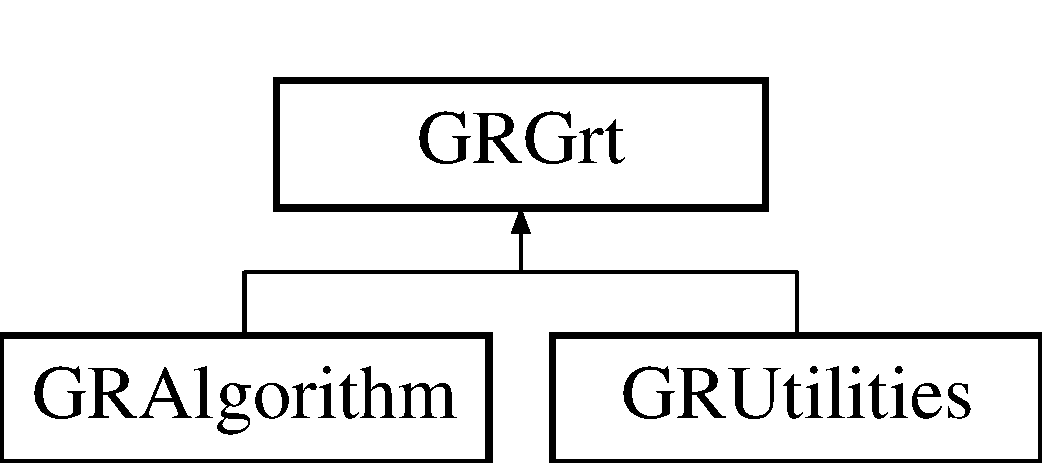
\includegraphics[height=2.000000cm]{classGRGrt}
\end{center}
\end{figure}
\subsection*{Public Member Functions}
\begin{DoxyCompactItemize}
\item 
\mbox{\Hypertarget{classGRGrt_aa6510bae51d0f3d2c6af5ee3852cff38}\label{classGRGrt_aa6510bae51d0f3d2c6af5ee3852cff38}} 
{\bfseries G\+R\+Grt} (const \mbox{\hyperlink{classGRGrt}{G\+R\+Grt}} \&)
\item 
\mbox{\Hypertarget{classGRGrt_ac386df585523d57c0f45eab413075b3f}\label{classGRGrt_ac386df585523d57c0f45eab413075b3f}} 
\mbox{\hyperlink{classGRGrt}{G\+R\+Grt}} \& {\bfseries operator=} (const \mbox{\hyperlink{classGRGrt}{G\+R\+Grt}} \&)
\item 
\mbox{\Hypertarget{classGRGrt_a734acc0c43d8a1a326c8107f1b5d8ed3}\label{classGRGrt_a734acc0c43d8a1a326c8107f1b5d8ed3}} 
bool {\bfseries load\+Training\+Data} (std\+::string filepath)
\item 
\mbox{\Hypertarget{classGRGrt_ac254a3cd3a2057665da563de0f763f87}\label{classGRGrt_ac254a3cd3a2057665da563de0f763f87}} 
bool {\bfseries load\+Test\+Data} (std\+::string filepath)
\item 
\mbox{\Hypertarget{classGRGrt_a9843133f434c214db226c4d5690113cb}\label{classGRGrt_a9843133f434c214db226c4d5690113cb}} 
bool {\bfseries set\+Test\+Data\+From\+Training} (int size)
\item 
\mbox{\Hypertarget{classGRGrt_a414538e216c5ab01569b11ddb27f3e16}\label{classGRGrt_a414538e216c5ab01569b11ddb27f3e16}} 
bool {\bfseries train} ()
\item 
\mbox{\Hypertarget{classGRGrt_a274708474e42eab554bf5056da63c231}\label{classGRGrt_a274708474e42eab554bf5056da63c231}} 
double {\bfseries test} ()
\item 
\mbox{\Hypertarget{classGRGrt_a1e78023522cece11f107d203ef3b1be7}\label{classGRGrt_a1e78023522cece11f107d203ef3b1be7}} 
double {\bfseries get\+Test\+Accuracy} ()
\item 
\mbox{\Hypertarget{classGRGrt_a20eb98bf5d0979c55cc4d91e1b191794}\label{classGRGrt_a20eb98bf5d0979c55cc4d91e1b191794}} 
bool {\bfseries save\+Model} (std\+::string filepath)
\item 
\mbox{\Hypertarget{classGRGrt_a09f32336a2b089dadbf1c6e72ee55f2a}\label{classGRGrt_a09f32336a2b089dadbf1c6e72ee55f2a}} 
bool {\bfseries load\+Model} (std\+::string filepath)
\item 
\mbox{\Hypertarget{classGRGrt_ae1ec1de504ebc34eb3f7d553ca683584}\label{classGRGrt_ae1ec1de504ebc34eb3f7d553ca683584}} 
bool {\bfseries predict} (G\+R\+T\+::\+Matrix\+Double timeseries)
\item 
\mbox{\Hypertarget{classGRGrt_a12807c23f6559c9b90d37b97fd07d07a}\label{classGRGrt_a12807c23f6559c9b90d37b97fd07d07a}} 
G\+R\+T\+::\+U\+I\+NT {\bfseries get\+Predicted\+Class\+Label} ()
\item 
\mbox{\Hypertarget{classGRGrt_ae8d858e1ffb1c1bebed87998bb0d094f}\label{classGRGrt_ae8d858e1ffb1c1bebed87998bb0d094f}} 
double {\bfseries get\+Maximum\+Likelihood} ()
\item 
\mbox{\Hypertarget{classGRGrt_a6e6807059279def6202e89904fe2704e}\label{classGRGrt_a6e6807059279def6202e89904fe2704e}} 
void {\bfseries set\+Dataset\+Properties} (std\+::string, std\+::string, std\+::string, int)
\item 
\mbox{\Hypertarget{classGRGrt_adca61031b452e7a1105a8755322c7120}\label{classGRGrt_adca61031b452e7a1105a8755322c7120}} 
void {\bfseries set\+Next\+Label} ()
\item 
\mbox{\Hypertarget{classGRGrt_a29bc0a4af10d5a97022c020e69ae14c9}\label{classGRGrt_a29bc0a4af10d5a97022c020e69ae14c9}} 
void {\bfseries clear\+Training\+Data} ()
\item 
\mbox{\Hypertarget{classGRGrt_afbd9af81bc8115a14ad069760c4812ce}\label{classGRGrt_afbd9af81bc8115a14ad069760c4812ce}} 
bool {\bfseries add\+Sample} (std\+::vector$<$ double $>$ $\ast$, std\+::vector$<$ double $>$ $\ast$)
\item 
\mbox{\Hypertarget{classGRGrt_ae8b794a630026859046d207d11e9c278}\label{classGRGrt_ae8b794a630026859046d207d11e9c278}} 
bool {\bfseries push\+Gesture} ()
\item 
\mbox{\Hypertarget{classGRGrt_a32cc6ef6833fe314702451731a8aee10}\label{classGRGrt_a32cc6ef6833fe314702451731a8aee10}} 
bool {\bfseries save\+Dataset} ()
\end{DoxyCompactItemize}


The documentation for this class was generated from the following file\+:\begin{DoxyCompactItemize}
\item 
/home/vlad/projects/brainhub/gestus\+S\+D\+K/inc/gr\+Grt.\+h\end{DoxyCompactItemize}

\hypertarget{classGRMadgwick}{}\section{G\+R\+Madgwick Class Reference}
\label{classGRMadgwick}\index{G\+R\+Madgwick@{G\+R\+Madgwick}}
\subsection*{Public Member Functions}
\begin{DoxyCompactItemize}
\item 
\mbox{\Hypertarget{classGRMadgwick_abb56985d4f31d3a19072df3c4c68d747}\label{classGRMadgwick_abb56985d4f31d3a19072df3c4c68d747}} 
{\bfseries G\+R\+Madgwick} (const \mbox{\hyperlink{classGRMadgwick}{G\+R\+Madgwick}} \&)
\item 
\mbox{\Hypertarget{classGRMadgwick_a0f73be02b42695bb4cc811d0966f19c9}\label{classGRMadgwick_a0f73be02b42695bb4cc811d0966f19c9}} 
\mbox{\hyperlink{classGRMadgwick}{G\+R\+Madgwick}} \& {\bfseries operator=} (const \mbox{\hyperlink{classGRMadgwick}{G\+R\+Madgwick}} \&)
\item 
\mbox{\Hypertarget{classGRMadgwick_a3975b7b1fb251e9cc05ee0817c7a9179}\label{classGRMadgwick_a3975b7b1fb251e9cc05ee0817c7a9179}} 
void {\bfseries Madgwick\+A\+H\+R\+Supdate} (double gx, double gy, double gz, double ax, double ay, double az, double mx, double my, double mz, std\+::vector$<$ double $>$ $\ast$)
\item 
\mbox{\Hypertarget{classGRMadgwick_a23586708a657d6b168facbd9e21571c8}\label{classGRMadgwick_a23586708a657d6b168facbd9e21571c8}} 
void {\bfseries Madgwick\+A\+H\+R\+Supdate\+I\+MU} (double gx, double gy, double gz, double ax, double ay, double az, std\+::vector$<$ double $>$ $\ast$)
\item 
\mbox{\Hypertarget{classGRMadgwick_ab38270f0bf98485f700bebb8df813d1c}\label{classGRMadgwick_ab38270f0bf98485f700bebb8df813d1c}} 
bool {\bfseries set\+Freq\+Calibration} (int)
\end{DoxyCompactItemize}


The documentation for this class was generated from the following file\+:\begin{DoxyCompactItemize}
\item 
/home/vlad/projects/brainhub/gestus\+S\+D\+K/inc/gr\+Madgwick.\+h\end{DoxyCompactItemize}

\hypertarget{classGRTrajectory}{}\section{G\+R\+Trajectory Class Reference}
\label{classGRTrajectory}\index{G\+R\+Trajectory@{G\+R\+Trajectory}}
\subsection*{Public Member Functions}
\begin{DoxyCompactItemize}
\item 
\mbox{\Hypertarget{classGRTrajectory_aae41cdeef895b295e27bcf07a64d6307}\label{classGRTrajectory_aae41cdeef895b295e27bcf07a64d6307}} 
std\+::vector$<$ double $>$ {\bfseries get\+New\+Pos\+By\+Runge} (std\+::vector$<$ double $>$, std\+::vector$<$ double $>$, unsigned long)
\item 
\mbox{\Hypertarget{classGRTrajectory_a2d6f58c0c68aeb6f0b0f20a082934789}\label{classGRTrajectory_a2d6f58c0c68aeb6f0b0f20a082934789}} 
std\+::vector$<$ double $>$ {\bfseries get\+Accelerations} (std\+::vector$<$ double $>$, std\+::vector$<$ double $>$)
\end{DoxyCompactItemize}


The documentation for this class was generated from the following file\+:\begin{DoxyCompactItemize}
\item 
/home/vlad/projects/brainhub/gestus\+S\+D\+K/inc/gr\+Trajectory.\+h\end{DoxyCompactItemize}

\hypertarget{classGRUtilities}{}\section{G\+R\+Utilities Class Reference}
\label{classGRUtilities}\index{G\+R\+Utilities@{G\+R\+Utilities}}
Inheritance diagram for G\+R\+Utilities\+:\begin{figure}[H]
\begin{center}
\leavevmode
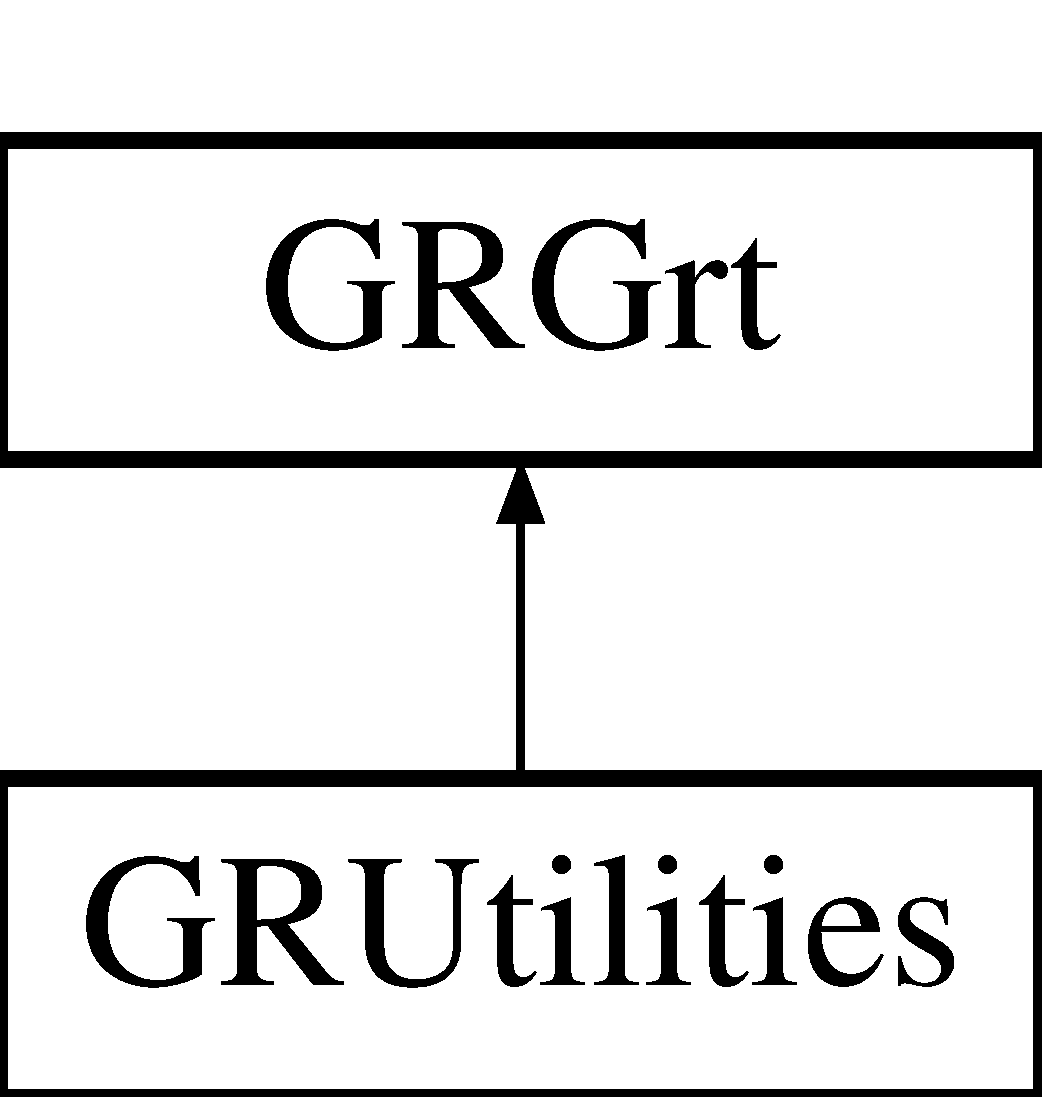
\includegraphics[height=2.000000cm]{classGRUtilities}
\end{center}
\end{figure}
\subsection*{Public Member Functions}
\begin{DoxyCompactItemize}
\item 
\mbox{\Hypertarget{classGRUtilities_a0d5634b33b4356e446d2ab1ef7a3f749}\label{classGRUtilities_a0d5634b33b4356e446d2ab1ef7a3f749}} 
{\bfseries G\+R\+Utilities} (const \mbox{\hyperlink{classGRUtilities}{G\+R\+Utilities}} \&)
\item 
\mbox{\Hypertarget{classGRUtilities_a12f50039407684c56b4ece2c6f48aad4}\label{classGRUtilities_a12f50039407684c56b4ece2c6f48aad4}} 
\mbox{\hyperlink{classGRUtilities}{G\+R\+Utilities}} \& {\bfseries operator=} (const \mbox{\hyperlink{classGRUtilities}{G\+R\+Utilities}} \&)
\end{DoxyCompactItemize}


The documentation for this class was generated from the following file\+:\begin{DoxyCompactItemize}
\item 
/home/vlad/projects/brainhub/gestus\+S\+D\+K/inc/gr\+Utilities.\+h\end{DoxyCompactItemize}

\hypertarget{structimu}{}\section{imu Struct Reference}
\label{structimu}\index{imu@{imu}}
\subsection*{Public Member Functions}
\begin{DoxyCompactItemize}
\item 
\mbox{\Hypertarget{structimu_aad015d789f4184b8e3f398a910965947}\label{structimu_aad015d789f4184b8e3f398a910965947}} 
bool {\bfseries empty} ()
\item 
\mbox{\Hypertarget{structimu_a3ca47098c4c0902a2ee226651ab4f1c3}\label{structimu_a3ca47098c4c0902a2ee226651ab4f1c3}} 
bool {\bfseries is\+\_\+complite} ()
\item 
\mbox{\Hypertarget{structimu_aca06ac68ca554729d999dd1bc2a36d24}\label{structimu_aca06ac68ca554729d999dd1bc2a36d24}} 
bool {\bfseries clear} ()
\end{DoxyCompactItemize}
\subsection*{Public Attributes}
\begin{DoxyCompactItemize}
\item 
\mbox{\Hypertarget{structimu_aba52b1213ab81c45af29454ea9ca7805}\label{structimu_aba52b1213ab81c45af29454ea9ca7805}} 
std\+::vector$<$ double $>$ {\bfseries gyro}
\item 
\mbox{\Hypertarget{structimu_adac97b95e4d1161816b78ff3ff14dddb}\label{structimu_adac97b95e4d1161816b78ff3ff14dddb}} 
std\+::vector$<$ double $>$ {\bfseries acc}
\item 
\mbox{\Hypertarget{structimu_aa5f359719d5d8c7dfac625dfe91de6cf}\label{structimu_aa5f359719d5d8c7dfac625dfe91de6cf}} 
std\+::vector$<$ double $>$ {\bfseries mag}
\item 
\mbox{\Hypertarget{structimu_a6700c732f9a576450518747e4e74826e}\label{structimu_a6700c732f9a576450518747e4e74826e}} 
unsigned long {\bfseries time\+\_\+stamp}
\item 
\mbox{\Hypertarget{structimu_a6d3d551ec276f287dede0b8f496027e3}\label{structimu_a6d3d551ec276f287dede0b8f496027e3}} 
bool {\bfseries is\+\_\+connected}
\end{DoxyCompactItemize}


The documentation for this struct was generated from the following file\+:\begin{DoxyCompactItemize}
\item 
/home/vlad/projects/brainhub/gestus\+S\+D\+K/inc/gr\+Device.\+h\end{DoxyCompactItemize}

\hypertarget{structk__filter__vars}{}\section{k\+\_\+filter\+\_\+vars Struct Reference}
\label{structk__filter__vars}\index{k\+\_\+filter\+\_\+vars@{k\+\_\+filter\+\_\+vars}}
\subsection*{Public Attributes}
\begin{DoxyCompactItemize}
\item 
\mbox{\Hypertarget{structk__filter__vars_a48ef9e5caf126fdcc048c7efef026ec0}\label{structk__filter__vars_a48ef9e5caf126fdcc048c7efef026ec0}} 
double {\bfseries volt}
\item 
\mbox{\Hypertarget{structk__filter__vars_a5fc0ab443a992ef71683d24e8a78633d}\label{structk__filter__vars_a5fc0ab443a992ef71683d24e8a78633d}} 
double {\bfseries proccess}
\item 
\mbox{\Hypertarget{structk__filter__vars_aa162ea5584bb45499cc4665a6b7d5fb7}\label{structk__filter__vars_aa162ea5584bb45499cc4665a6b7d5fb7}} 
double {\bfseries pc}
\item 
\mbox{\Hypertarget{structk__filter__vars_af6fae8f53161a6acc7819c2d99258217}\label{structk__filter__vars_af6fae8f53161a6acc7819c2d99258217}} 
double {\bfseries g}
\item 
\mbox{\Hypertarget{structk__filter__vars_a04840d6f95607d07e6fcf78cdba82a5e}\label{structk__filter__vars_a04840d6f95607d07e6fcf78cdba82a5e}} 
double {\bfseries p}
\item 
\mbox{\Hypertarget{structk__filter__vars_a73557b4cfe4e835995befe8c6d2747a2}\label{structk__filter__vars_a73557b4cfe4e835995befe8c6d2747a2}} 
double {\bfseries xp}
\item 
\mbox{\Hypertarget{structk__filter__vars_a156b05932418980070b9cc0c61b342bd}\label{structk__filter__vars_a156b05932418980070b9cc0c61b342bd}} 
double {\bfseries zp}
\item 
\mbox{\Hypertarget{structk__filter__vars_a96c7ee8ecb897cf118b9ab4da55dd9ba}\label{structk__filter__vars_a96c7ee8ecb897cf118b9ab4da55dd9ba}} 
double {\bfseries xe}
\item 
\mbox{\Hypertarget{structk__filter__vars_aedef0f703f2400924438514938ebfae0}\label{structk__filter__vars_aedef0f703f2400924438514938ebfae0}} 
std\+::vector$<$ double $>$ {\bfseries accumulated}
\end{DoxyCompactItemize}


The documentation for this struct was generated from the following file\+:\begin{DoxyCompactItemize}
\item 
/home/vlad/projects/brainhub/gestus\+S\+D\+K/inc/gr\+Algorithm.\+h\end{DoxyCompactItemize}

\hypertarget{structrunge__vars}{}\section{runge\+\_\+vars Struct Reference}
\label{structrunge__vars}\index{runge\+\_\+vars@{runge\+\_\+vars}}
\subsection*{Public Attributes}
\begin{DoxyCompactItemize}
\item 
\mbox{\Hypertarget{structrunge__vars_a89b75da82b2a1c1237296fb7c33e8b93}\label{structrunge__vars_a89b75da82b2a1c1237296fb7c33e8b93}} 
Eigen\+::\+Vector3d {\bfseries vel} = Eigen\+::\+Vector3d(0.f, 0.f, 0.f)
\item 
\mbox{\Hypertarget{structrunge__vars_a0ab2daf75798374698b54eef912fed78}\label{structrunge__vars_a0ab2daf75798374698b54eef912fed78}} 
Eigen\+::\+Vector3d {\bfseries pos} = Eigen\+::\+Vector3d(0.f, 0.f, 0.f)
\item 
\mbox{\Hypertarget{structrunge__vars_ad4d7394fcb60cc68782af14aea77188a}\label{structrunge__vars_ad4d7394fcb60cc68782af14aea77188a}} 
Eigen\+::\+Vector3d {\bfseries acc} = Eigen\+::\+Vector3d(0.f, 0.f, 0.f)
\end{DoxyCompactItemize}


The documentation for this struct was generated from the following file\+:\begin{DoxyCompactItemize}
\item 
/home/vlad/projects/brainhub/gestus\+S\+D\+K/inc/gr\+Trajectory.\+h\end{DoxyCompactItemize}

%--- End generated contents ---

% Index
\backmatter
\newpage
\phantomsection
\clearemptydoublepage
\addcontentsline{toc}{chapter}{Index}
\printindex

\end{document}
